\section*{Usage Notes}
%%Brief instructions that may help other researchers reuse these dataset.
%%This is an optional section, but strongly encouraged when helpful
%%to readers. This may include discussion of software packages that
%%are suitable for analyzing the assay data files, suggested downstream
%%processing steps (e.g. normalization, etc.), or tips for integrating
%%or comparing this with other datasets. If needed, authors are encouraged
%%to provide code, programs, or data processing workflows when they may help 
%%others analyse the data. We encourage authors to archive related code in 
%%a DOI-issuing archive when possible, but code may also be supplied as 
%%supplementary information files. 
%%
%%For studies involving privacy or safety controls on public access
%%to the data, this section should describe in detail these controls,
%%including how authors can apply to access the data, and what criteria
%%will be used to determine who may access the data, and any limitations
%%on data use.

\subsubsection*{Standartox Filters}





\subsection*{Web application}

Users can define several input parameters \ref{tab:inputs} in the application's graphical user interface (GUI), handled in the ui.R script in order to adjust the aggregation according specific requirements. In doing so users execute R functions (fun\_filter.R, fun\_aggregation.R, fun\_filagg\_plot\_ly.R) loaded in the server.R script, which produce a 'filtered' and an 'aggregated' data set as well as an interactive overview plot. Only the 'aggregated' data set is presented in the GUI. However, both data sets can be downloaded via a download button.

\subsection*{R package}

The R-package standartox

\definecolor{dkgreen}{rgb}{0,0.6,0}
\definecolor{gray}{rgb}{0.5,0.5,0.5}
\definecolor{mauve}{rgb}{0.58,0,0.82}

\lstset{frame=tb,
  language=R,
  aboveskip=3mm,
  belowskip=3mm,
  showstringspaces=false,
  columns=flexible,
  basicstyle={\small\ttfamily},
  numbers=none,
  numberstyle=\tiny\color{gray},
  keywordstyle=\color{blue},
  commentstyle=\color{dkgreen},
  stringstyle=\color{mauve},
  breaklines=true,
  breakatwhitespace=true,
  tabsize=3
}

\begin{lstlisting}
# install
install.packages('remotes')
remotes::install_github('andschar/standartox') # package not yet on CRAN
# retrieve catalog    
require(standartox)
catal = stx_catalog()
# retrieve data
l = stx_query(cas = cas,
              endpoint = 'XX50',
              taxa = 'Oncorhynchus',
              duration = c(24, 120))
\end{lstlisting}





The \etoxbase{} is designed to support CRA of ecotoxicologists. With an increased amount of available ecotoxicological test data, it becomes fundamental to provide and distribute such information in reasonable formats, meaning accessible for humans as well as machines. Currently CRA often relies on test results of a few, well tested standard organism, such as \textit{Daphnia magna}, \textit{Pimephales promelas}, \textit{Selenastrum capricornutum}, although researchers have conducted experiments on a much greater variety of organisms (e.g. the 926,108 test results collected in the EPA ECOTOX data base). In order to locate ecotoxicological test data, researchers can rely on individual test results reported in publications <CITE>, on compiled and published data sets \citep{malaj_organic_2014} or on data bases such as the Pesticide Property Data Base (PPDB) \citep{lewis_international_2016}. Each data source has its limitations though: Collecting toxicity information from individual publications is laborious and using already compiled data from publications or data bases is often limited to a specific groups of chemicals, such as pesticides, biozides etc. The \etoxbase{}, making use of the EPA ECOTOX data base, the largest publicly available collection of ecotoxicological test results, aims to facilitate the data retrieval process by providing adequate aggregates (\ecfifty{}, NOEC, LOEC) of the tests results. These are then used for the calculation of SSDs, TUs or other risk indicators. SSDs try to extrapolate effects of chemicals towards organisms from species to a community level by fitting a statistical distribution to toxicity test results on organisms of different trophic levels in order to derive concentrations at which a specific fraction of organisms are effected (often at 5\% - HC\textsubscript{5} \citep{posthuma_species_2002}. Figure \ref{fig:ssd-isoproturon} shows an example of a SSD and the derived HC\textsubscript{5} value (red dassed line) created for the herbicide Isoproturon. TUs are another indicator of effects of chemicals on organisms. They are calculated by dividing a measured concentration (c) by an \ecfifty{} value (cf. Equation \ref{eq:tu}).

\begin{equation}
    TU_i = \frac{c_i}{\ecfifty}
    \label{eq:tu}
\end{equation}

\begin{figure}[h!]
    \dentering
    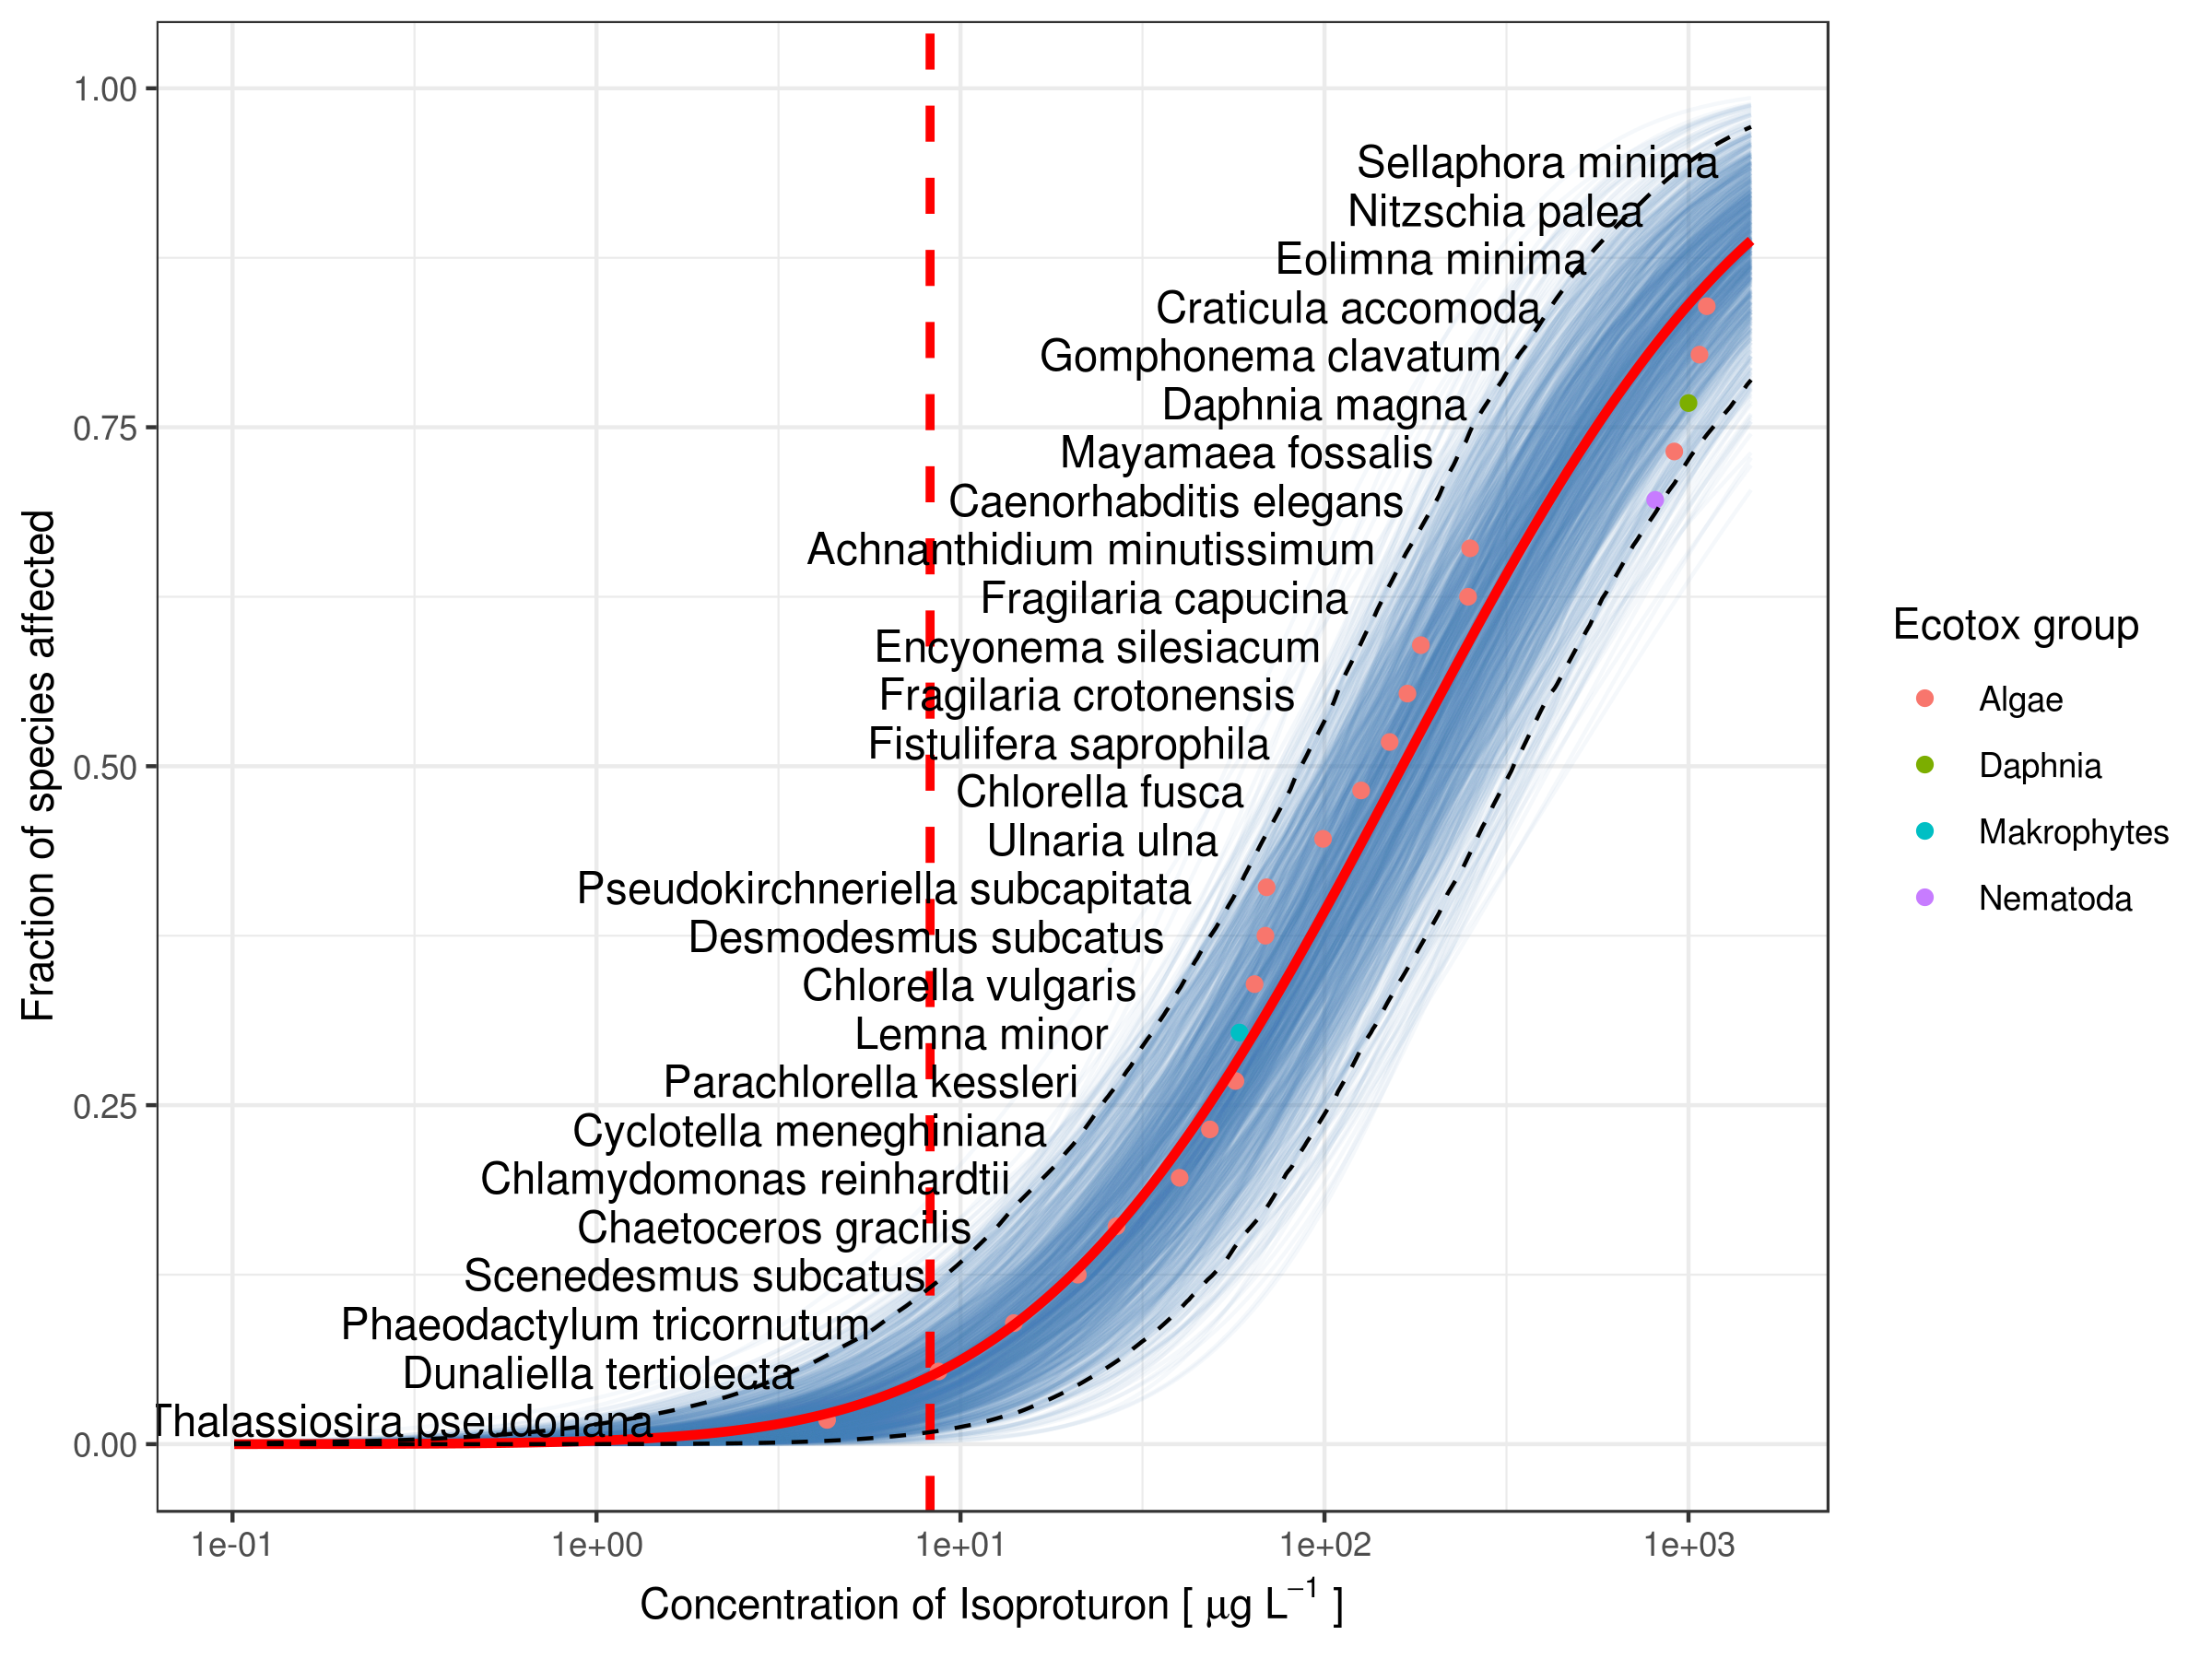
\includegraphics[width=1\linewidth]{article/figures/ssd2_boot.png}
    \caption{SSD plot showing the susceptibility of organisms towards the herbicide Isoproturon. The red line represents the fit and the red dashed line marks the HC\textsubscript{5} value, which is a common measure in CRA. The legend denotes common organism groups used in ecotoxicology.}
    \label{fig:ssd-isoproturon}
\end{figure}

\subsection*{Filter and Aggregate}

In the application's GUI, the user can choose among different parameters to filter and aggregate the test data accordingly \ref{tab:inputs}. Percentage values next to inputs show the proportion of the respective option (e.g. \textit{Active Ingredient - 43\%} indicates that 43\% of the data are Active Ingredients). The user can filter for compound-specific filters, including the CAS number, the concentration type (e.g. Active Ingredient, Formulation), the chemical class (e.g. Insecticides, Metals) and taxon-specific filters, including common taxonomic groups (e.g. Daphniidae, Algae), the organism habitat (e.g. freshwater) and the continent (e.g. Europe, Asia). Regarding the test parameters the user can choose test durations (in hours), Effect groups (e.g. Mortaliy, Population, Growth) and Endpoints (\ecfifty, EC\textsubscript{10}, LOEC or NOEC). Besides that, two cleaning steps can also be chosen. Firstly the application allows to exclude test results exhibiting concentrations that are higher than the actual water solubility of the respective chemical at \ang{20} C. Secondly the user can choose to exclude outliers (cf. Table \ref{tab:scripts-app}). The outliers are selected as values that exceed lower (0.25) and the upper (0.75) quartile by 1.5 times the inter-quartile range. As aggregates the user can choose the minimum, the maximum, the median, the geometric mean or the arithmetic mean. All the steps described in this section are selectable in the GUI and are executed at each click by the application. The drop down menu `Download data` allows to download a filtered data set as well as an aggregated data set.

\subsection*{Limitations}

Generally it has to be stated that the returned values are subject to change, as new tests will be constantly incorporated into the \etoxbase{}. However, we expect values of well tested chemical-organism combinations to be relatively stable. The returned values are certainly influenced by individual tests characteristics, such as pH, temperature or conductivity to just name a few, which influences the effect relationship between chemicals and organisms \citep{rosenkrantz_influence_2013,li_temperature_2011}. Unfortunately the EPA ECOTOX data base has only rare records on test parameters, which prevents incorporating such parameters in an aggregation <proportions of available data: Temperature:77\%, pH:56\%, hardness:27\%, dissolved oxygen:18\%, Alkalinity:15\%, salinity:9\%, others:<=5\%>. However, using the median or the geometric mean as an aggregate allows for an adequate estimation of the central tendency of the toxicity of a chemical towards an organism group. The geometric mean is recommended, as it is in comparison to the arithmetic mean considerably less influenced by outliers and is suitable for skewed data. Also, the geometric mean is preferable in contrast to the median, since the median completely ignores the influence of large or small values, making it unreliable for small data sets <CITATION GEOMETRIC MEAN>.

Other initiatives, with different, though partly overlapping aims accumulating existing ecotoxicological test data are published online. The PPDB provides validated ecotoxicological test results for pesticides, narrowing chemicals to this group \citep{lewis_international_2016}. The Network of reference laboratories, research centres and related organisations for monitoring of emerging environmental substances (NORMAN) focuses on assembling river basin specific pollutants\citep{von_der_ohe_new_2011}. The EnviroTox data base \href{https://envirotoxdatabase.org/} makes also use of the \epa{} data in order to derive Predicted no-effect concentrations (PNEC) \citep{health_and_environmental_sciences_institute_hesi_envirotox_2019}. In comparison to the \etoxbase, these examples partly rely on the same data, yet not aiming to derive \ecfifty, LOEC and NOEC from it automatically.
\subsection*{Other data bases}

Ecotox tool for PENEC
Lara's work for regulatory thresholds


greater and greater demand to numerically  analyse large amount of ecotoxicological data.

Other data bases are also thought of. Compare Sascha Bub's work.



\subsection*{Identify chemicals to be tested}

\begin{figure}
    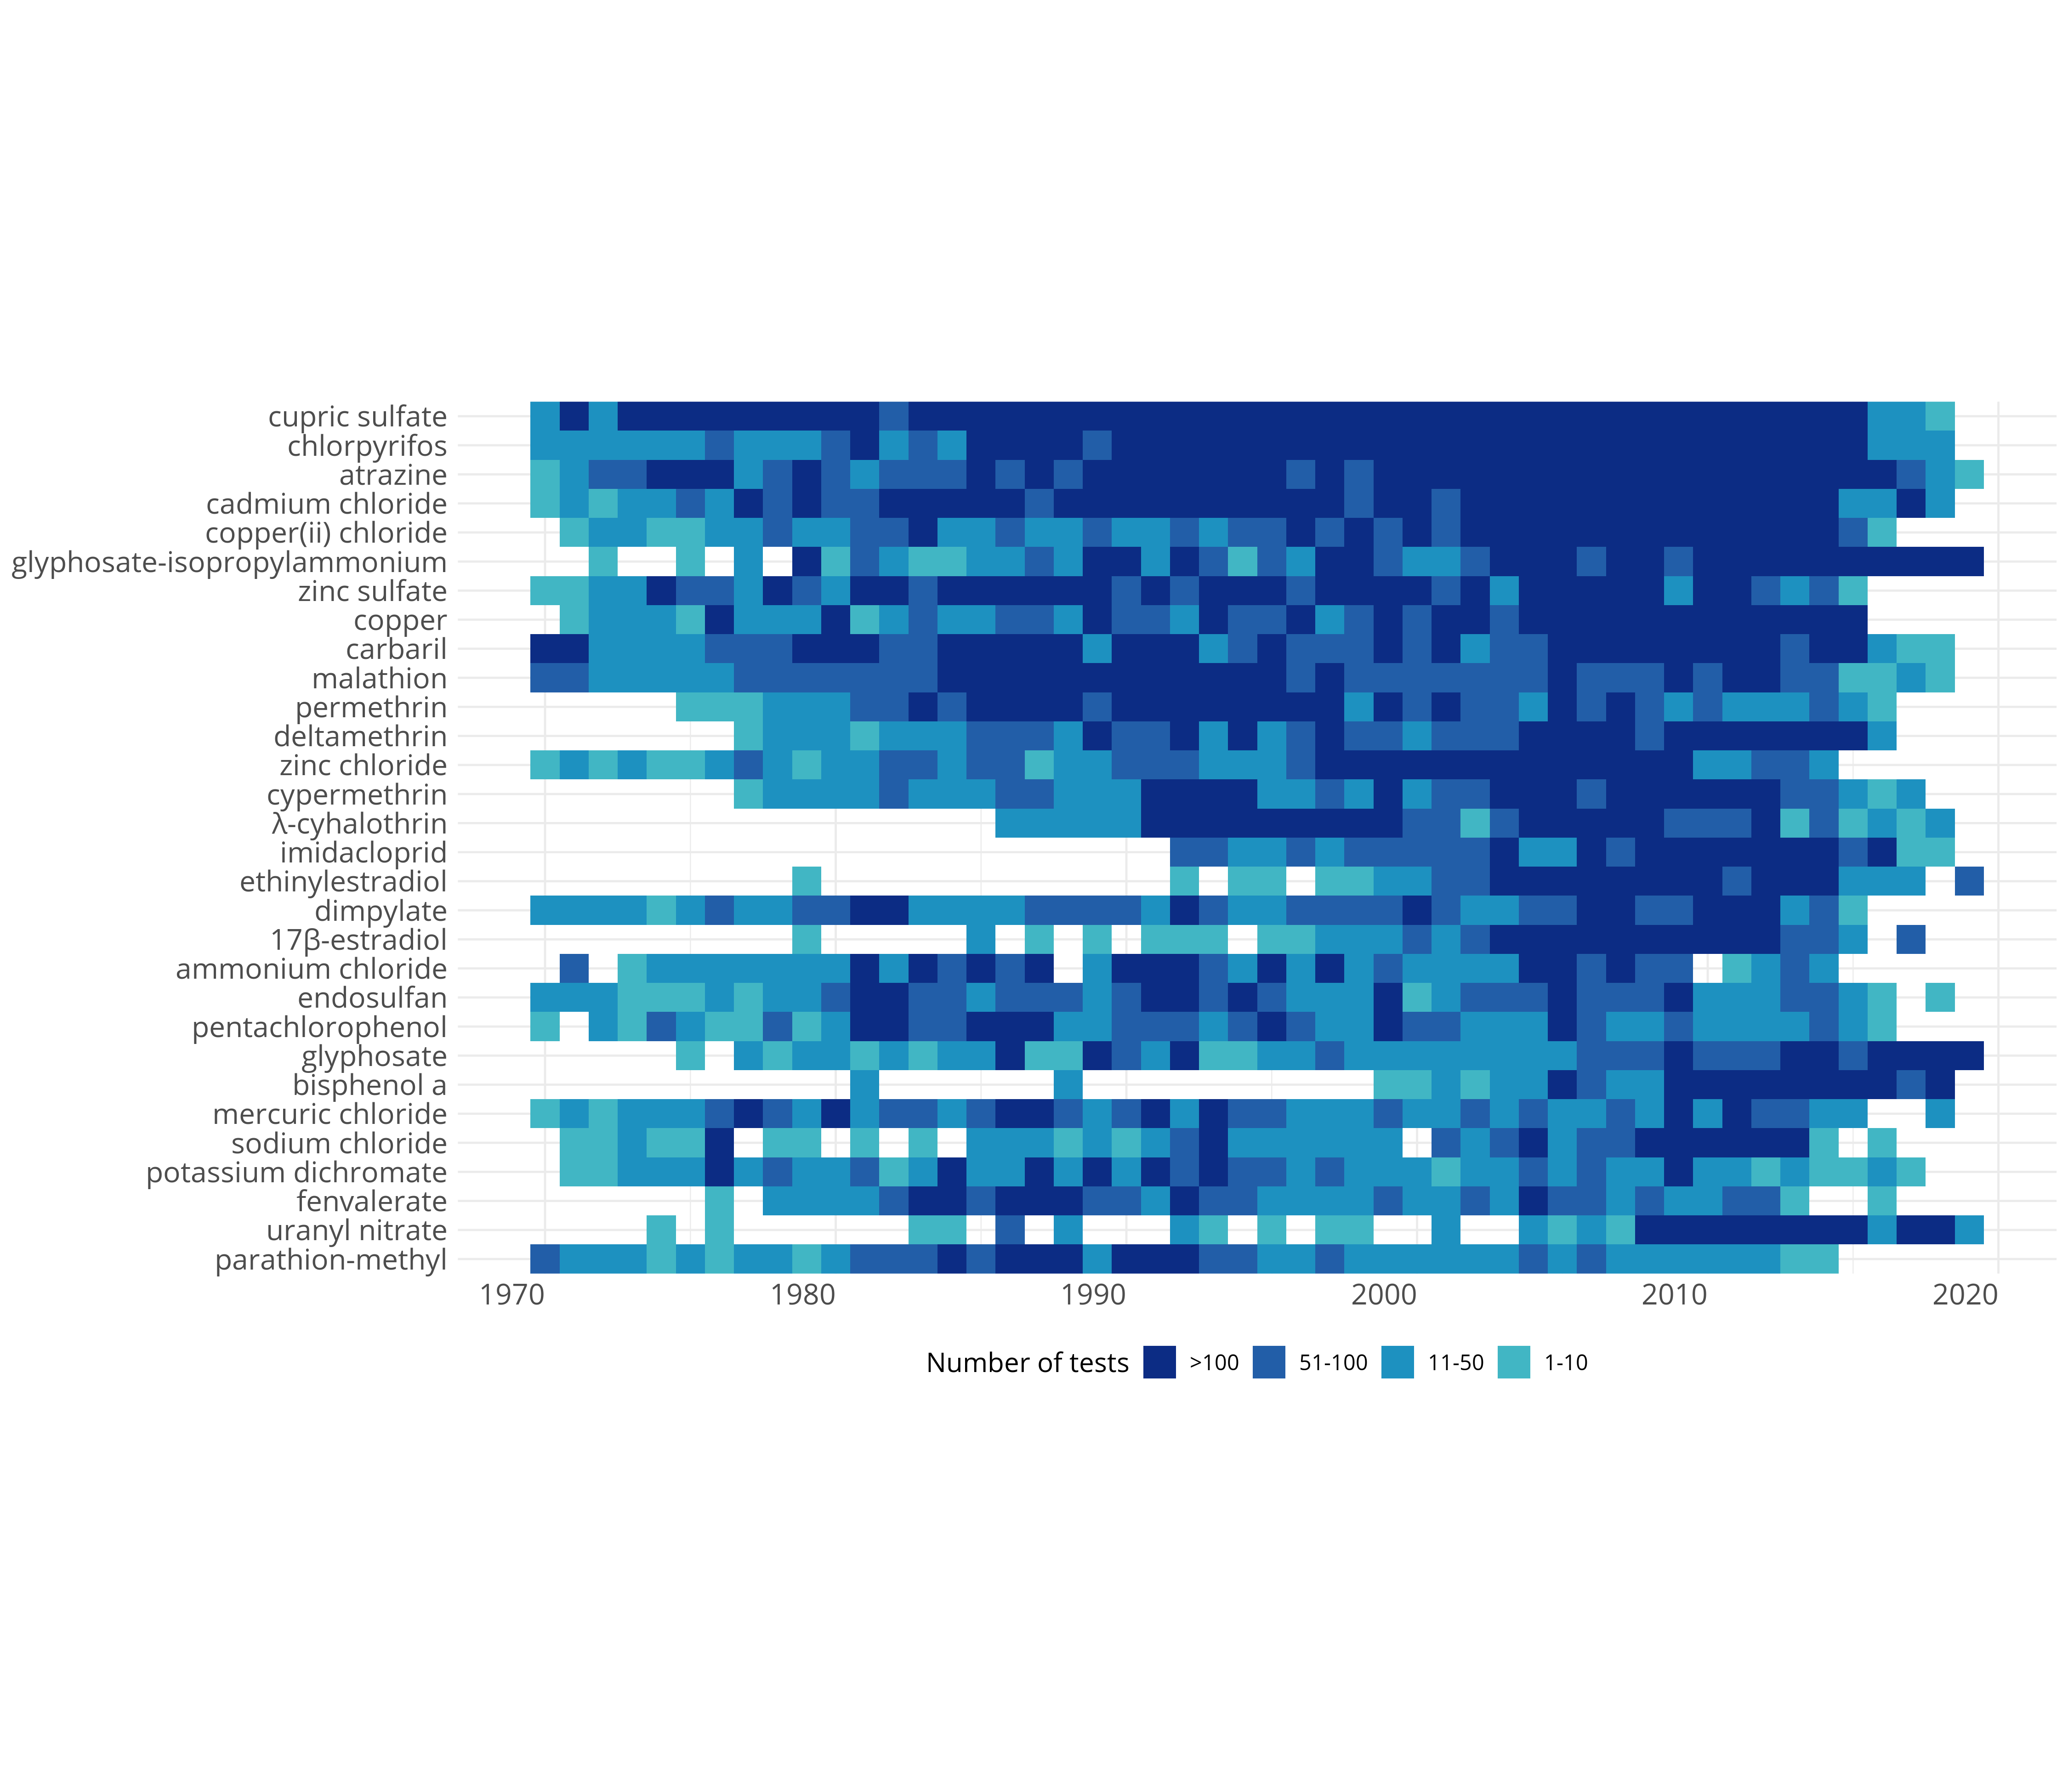
\includegraphics[width=1\linewidth]{article/figures/heatmap_tests_n.png}
    \caption{30 most tested chemicals in EPA ECOTOX.}
    \label{fig:standartox_ppdb_diff}
\end{figure}



There is a clear need in ecotoxicology for harmonised approaches to collect ecotoxicological data as other data base compilation attempts recently published show.

Hitchock et al. \citet{hitchcock_improving_2018} argue for an increased awareness concerning newly published ecotoxicological test results to facilitate meta analyses across studies. Important statistical parameters, such as mean estimates, variances ans sample sizes. Likewise, state variables, including medium temperature, pH, mineral contents or organism age and sex should be reported (if not in the text, in an online repository). Standartox doesn't include such information mainly because the EPA ECOTOX data base reports only a few of these variables. A future research aim could be to use machine learning techniques to retrieve this information from the referenced articles.

Agrochemicals contribute to a decline in biodiversity \citep{schafer_future_2019}
contrary to EU pesticide regulation

Current risk assessment or pesticide regulation consists of Stadard Toxicity Tests and Safety factors. They are not sufficient 

tiered framework critizized, especiall the two main assumptions:
(1) 1st tier provides and overly protective measure
(2) higher tiers provide more ecologically relevant predictions

"Inacurate predictions of exposure and effect" \citep{schafer_future_2019}

In their policy brief for a future risk assessment Schäfer et al. \citet{schafer_future_2019} propose to include a greater ecological context, meaning that not only single but communities need to evaluated and a landscape-oriented contemplation should be envisaged inter alia. Standartox partly follows such a route in making ecotoxicological data more easily available by standardizing ????? (1st tier) and integrating habitat and occurrence data, allowing for a more geographically detailed refinement.




Hallmann et al. \citet{hallmann_declines_2014} showed a decline of insectivorous birds associated with neonicotinoid usage.

Fungicides paper zitieren?






Standartox follows such a route in trying to synthesize information from a plethora of studies.






\pagebreak